While working on a project tree, the user must explicitly save the project tree for changes to be persisted to the database. This can be done by clicking on the "Save Project" button, as seen in the bottom left corner of the figure below

	\begin{figure}[H]
	    	\centering
	    	\fbox{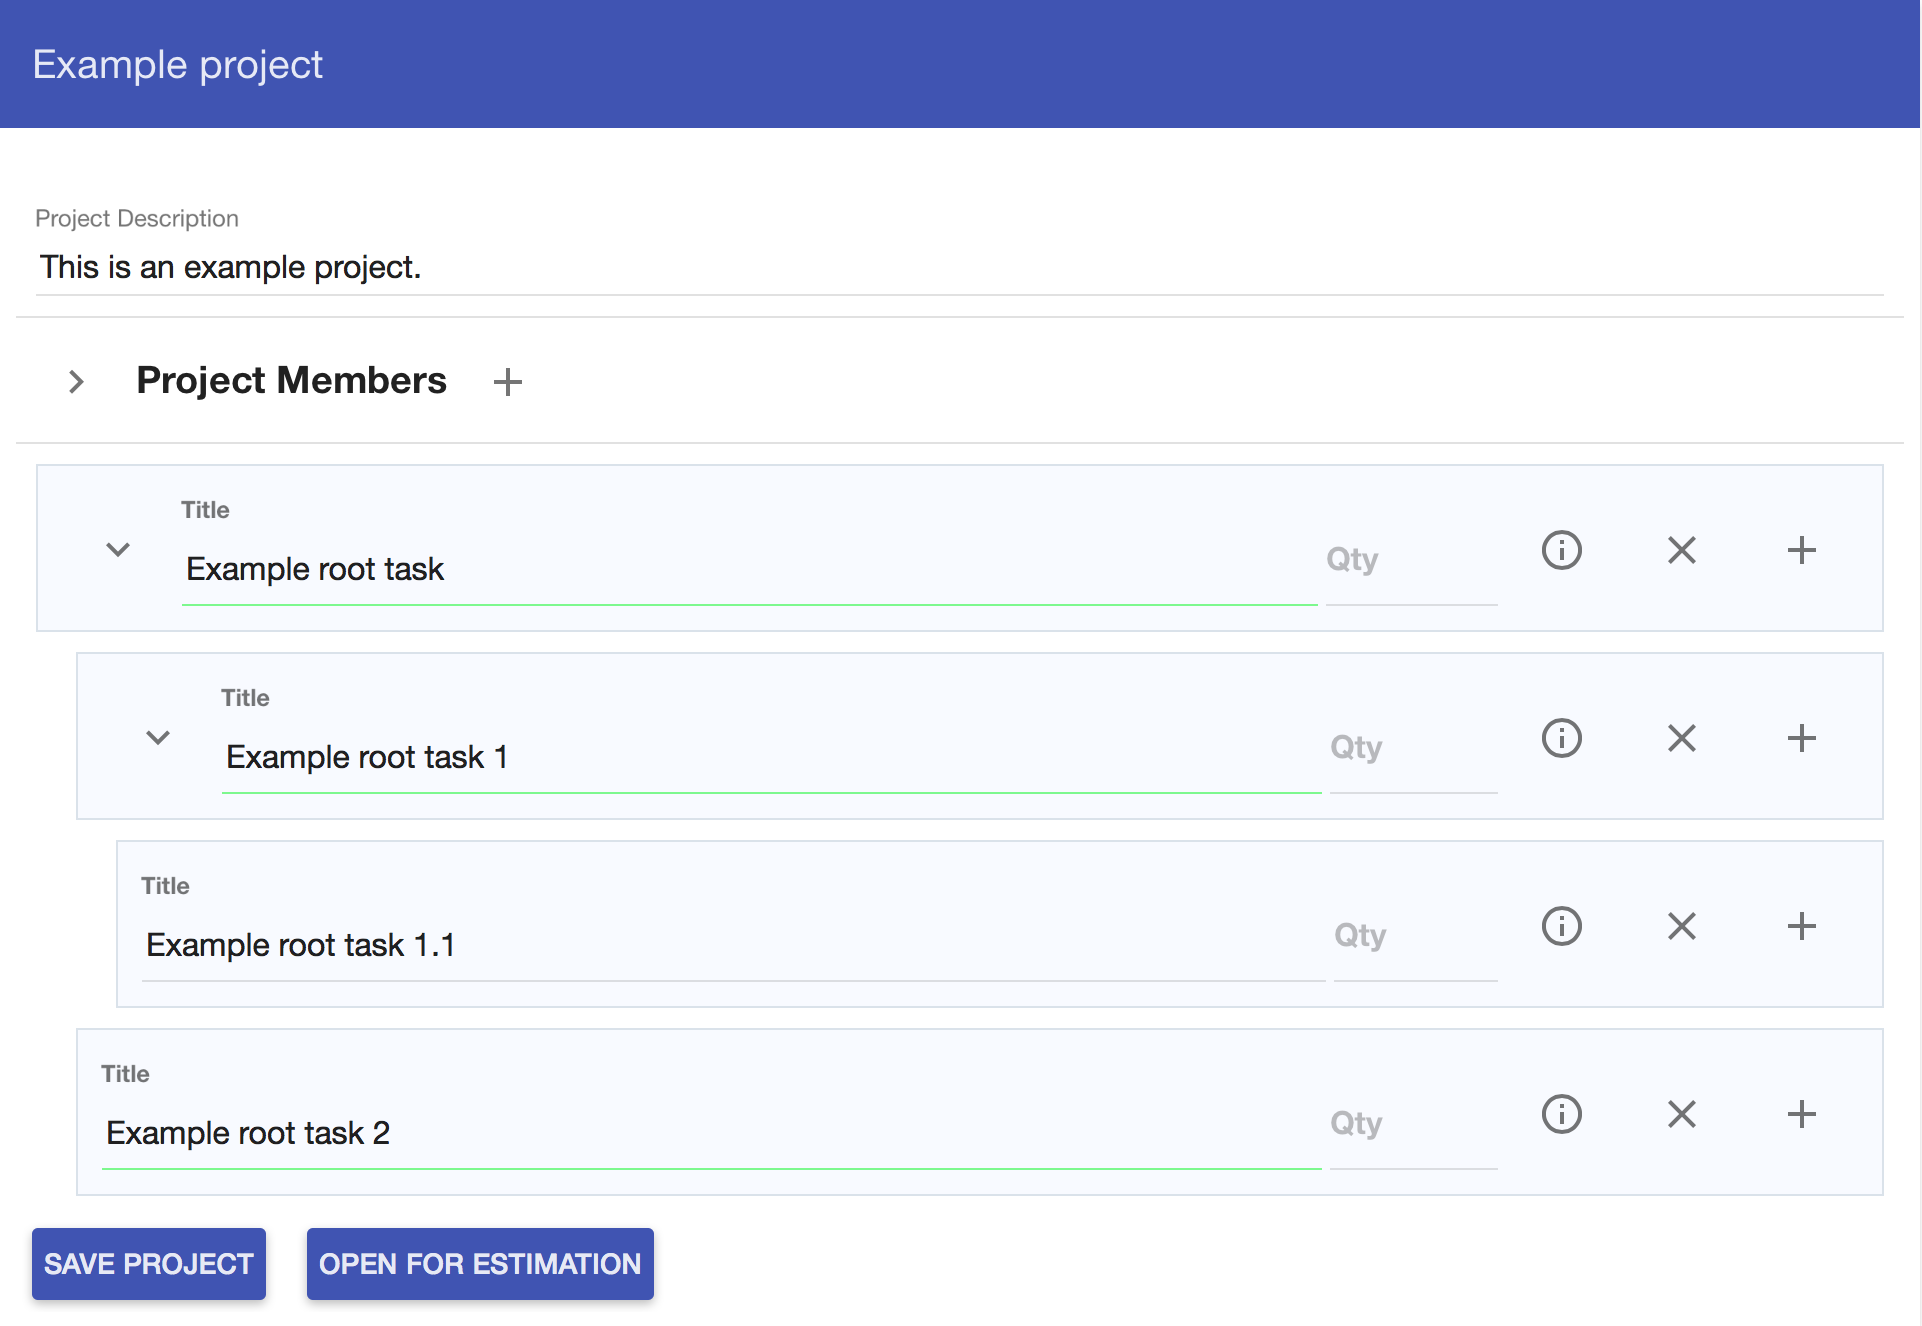
\includegraphics[width=0.5\textwidth]{saveProject}}
	    	\caption{Save Project}
	    	\label{fig: Save Project}
   	\end{figure}

If the user has not saved the project tree, and attempts to navigate away from the edit project page, the user will be prompted with the confirmation dialog displayed in the figure below.

	\begin{figure}[H]
	    	\centering
	    	\fbox{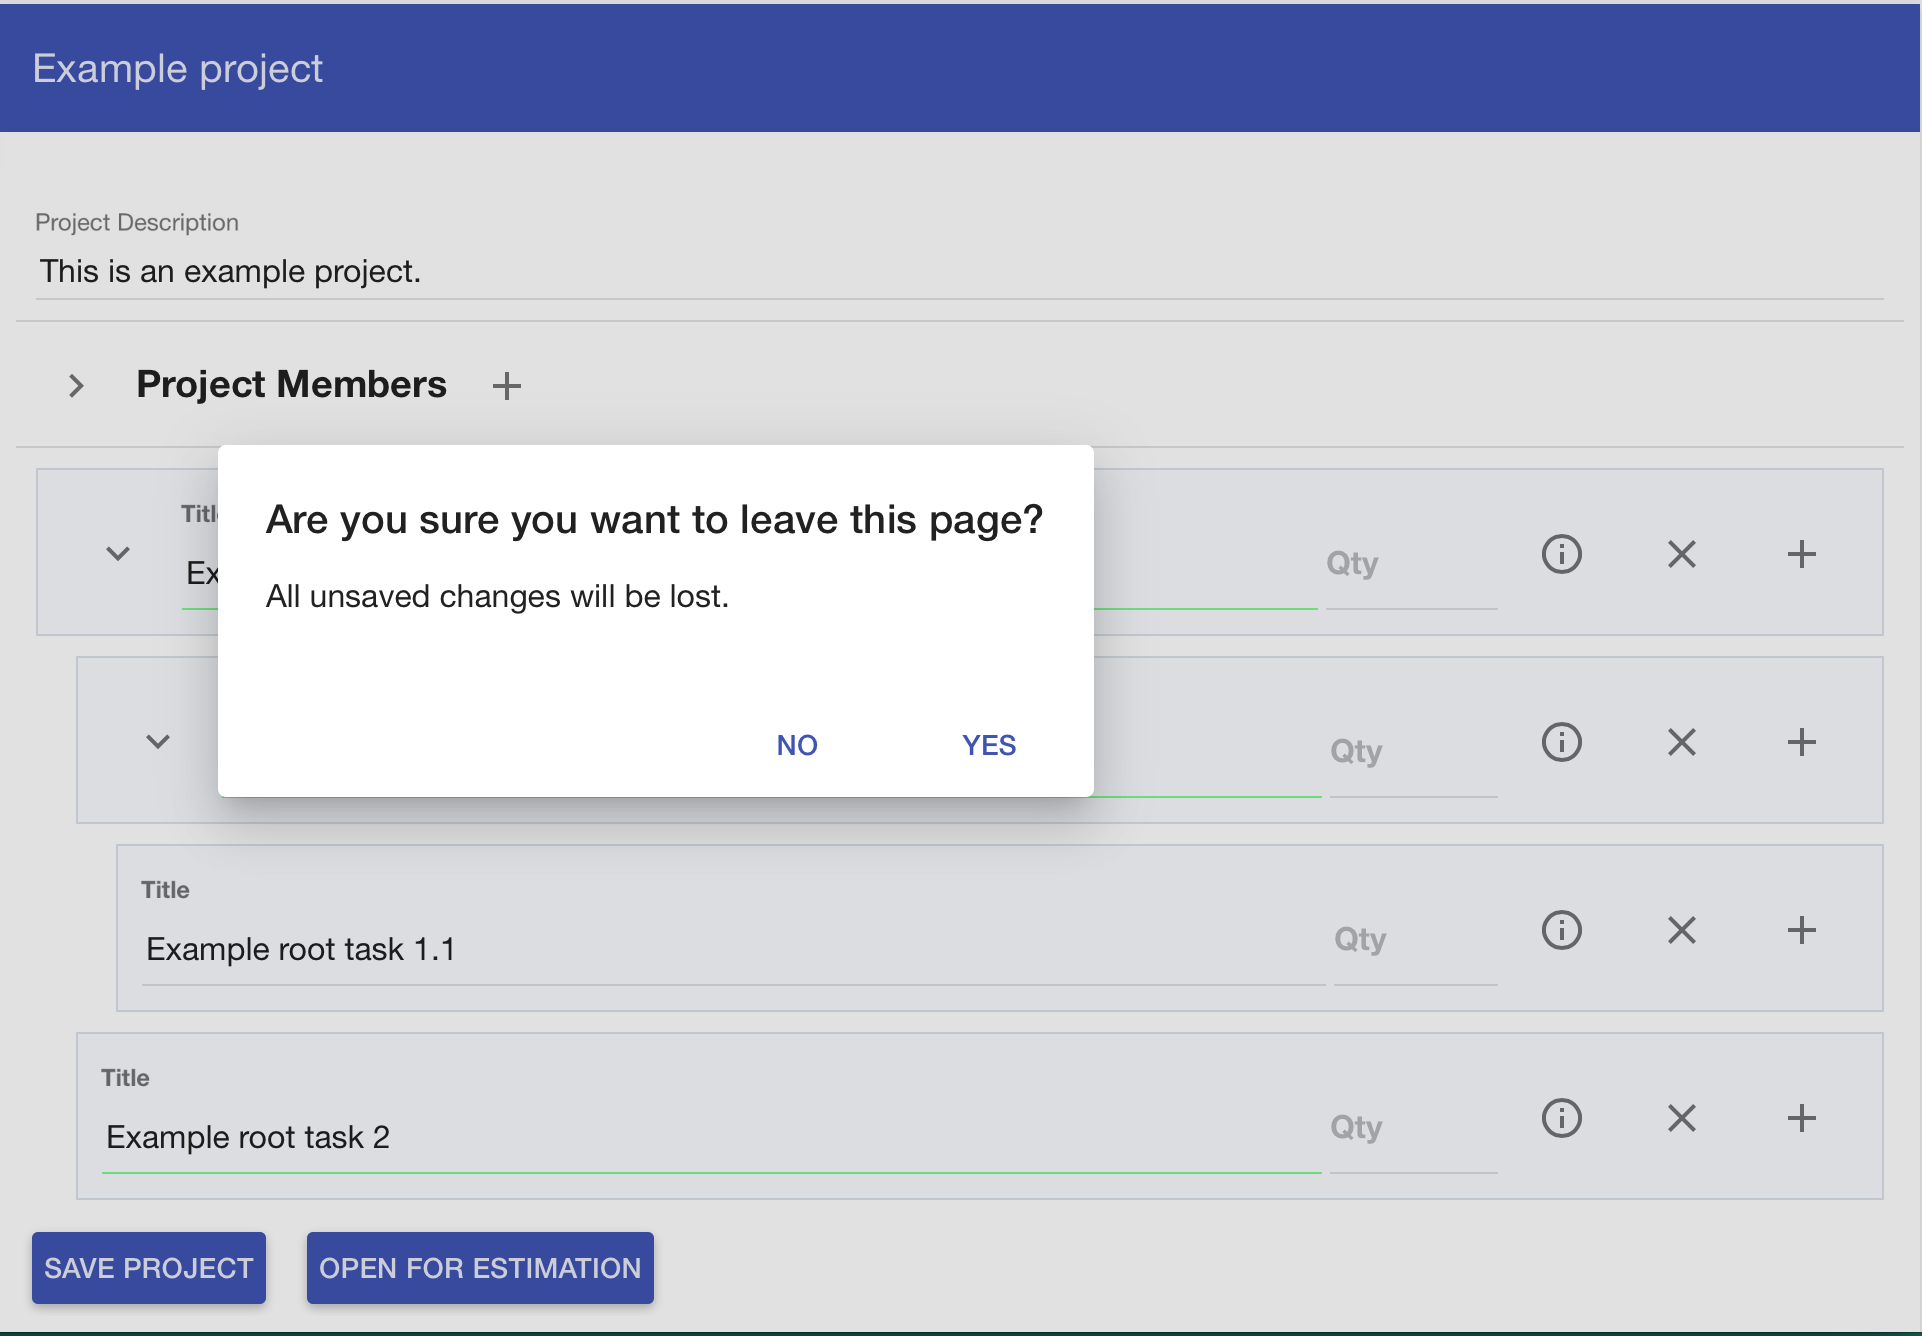
\includegraphics[width=0.5\textwidth]{confirmNavigateAway}}
	    	\caption{Confirmation of navigation away}
	    	\label{fig: Confirmation}
   	\end{figure}

If the user wishes to discard changes, he/she can navigate away from the page without saving the changes. Otherwise, the user can cancel the navigation process, and then save the project, and then continue to navigate away. A similar process is performed when a user is in the process of Estimation.
\subsection{Error Reporting}
Should you encounter a error or need some additional help do not hesitate to create a issues on the 
\href{https://github.com/FrikkieSnyman/COS301_GroupProject}{gitHub webpage} of the project.
	\begin{figure}[H]
	    	\centering
	    	\fbox{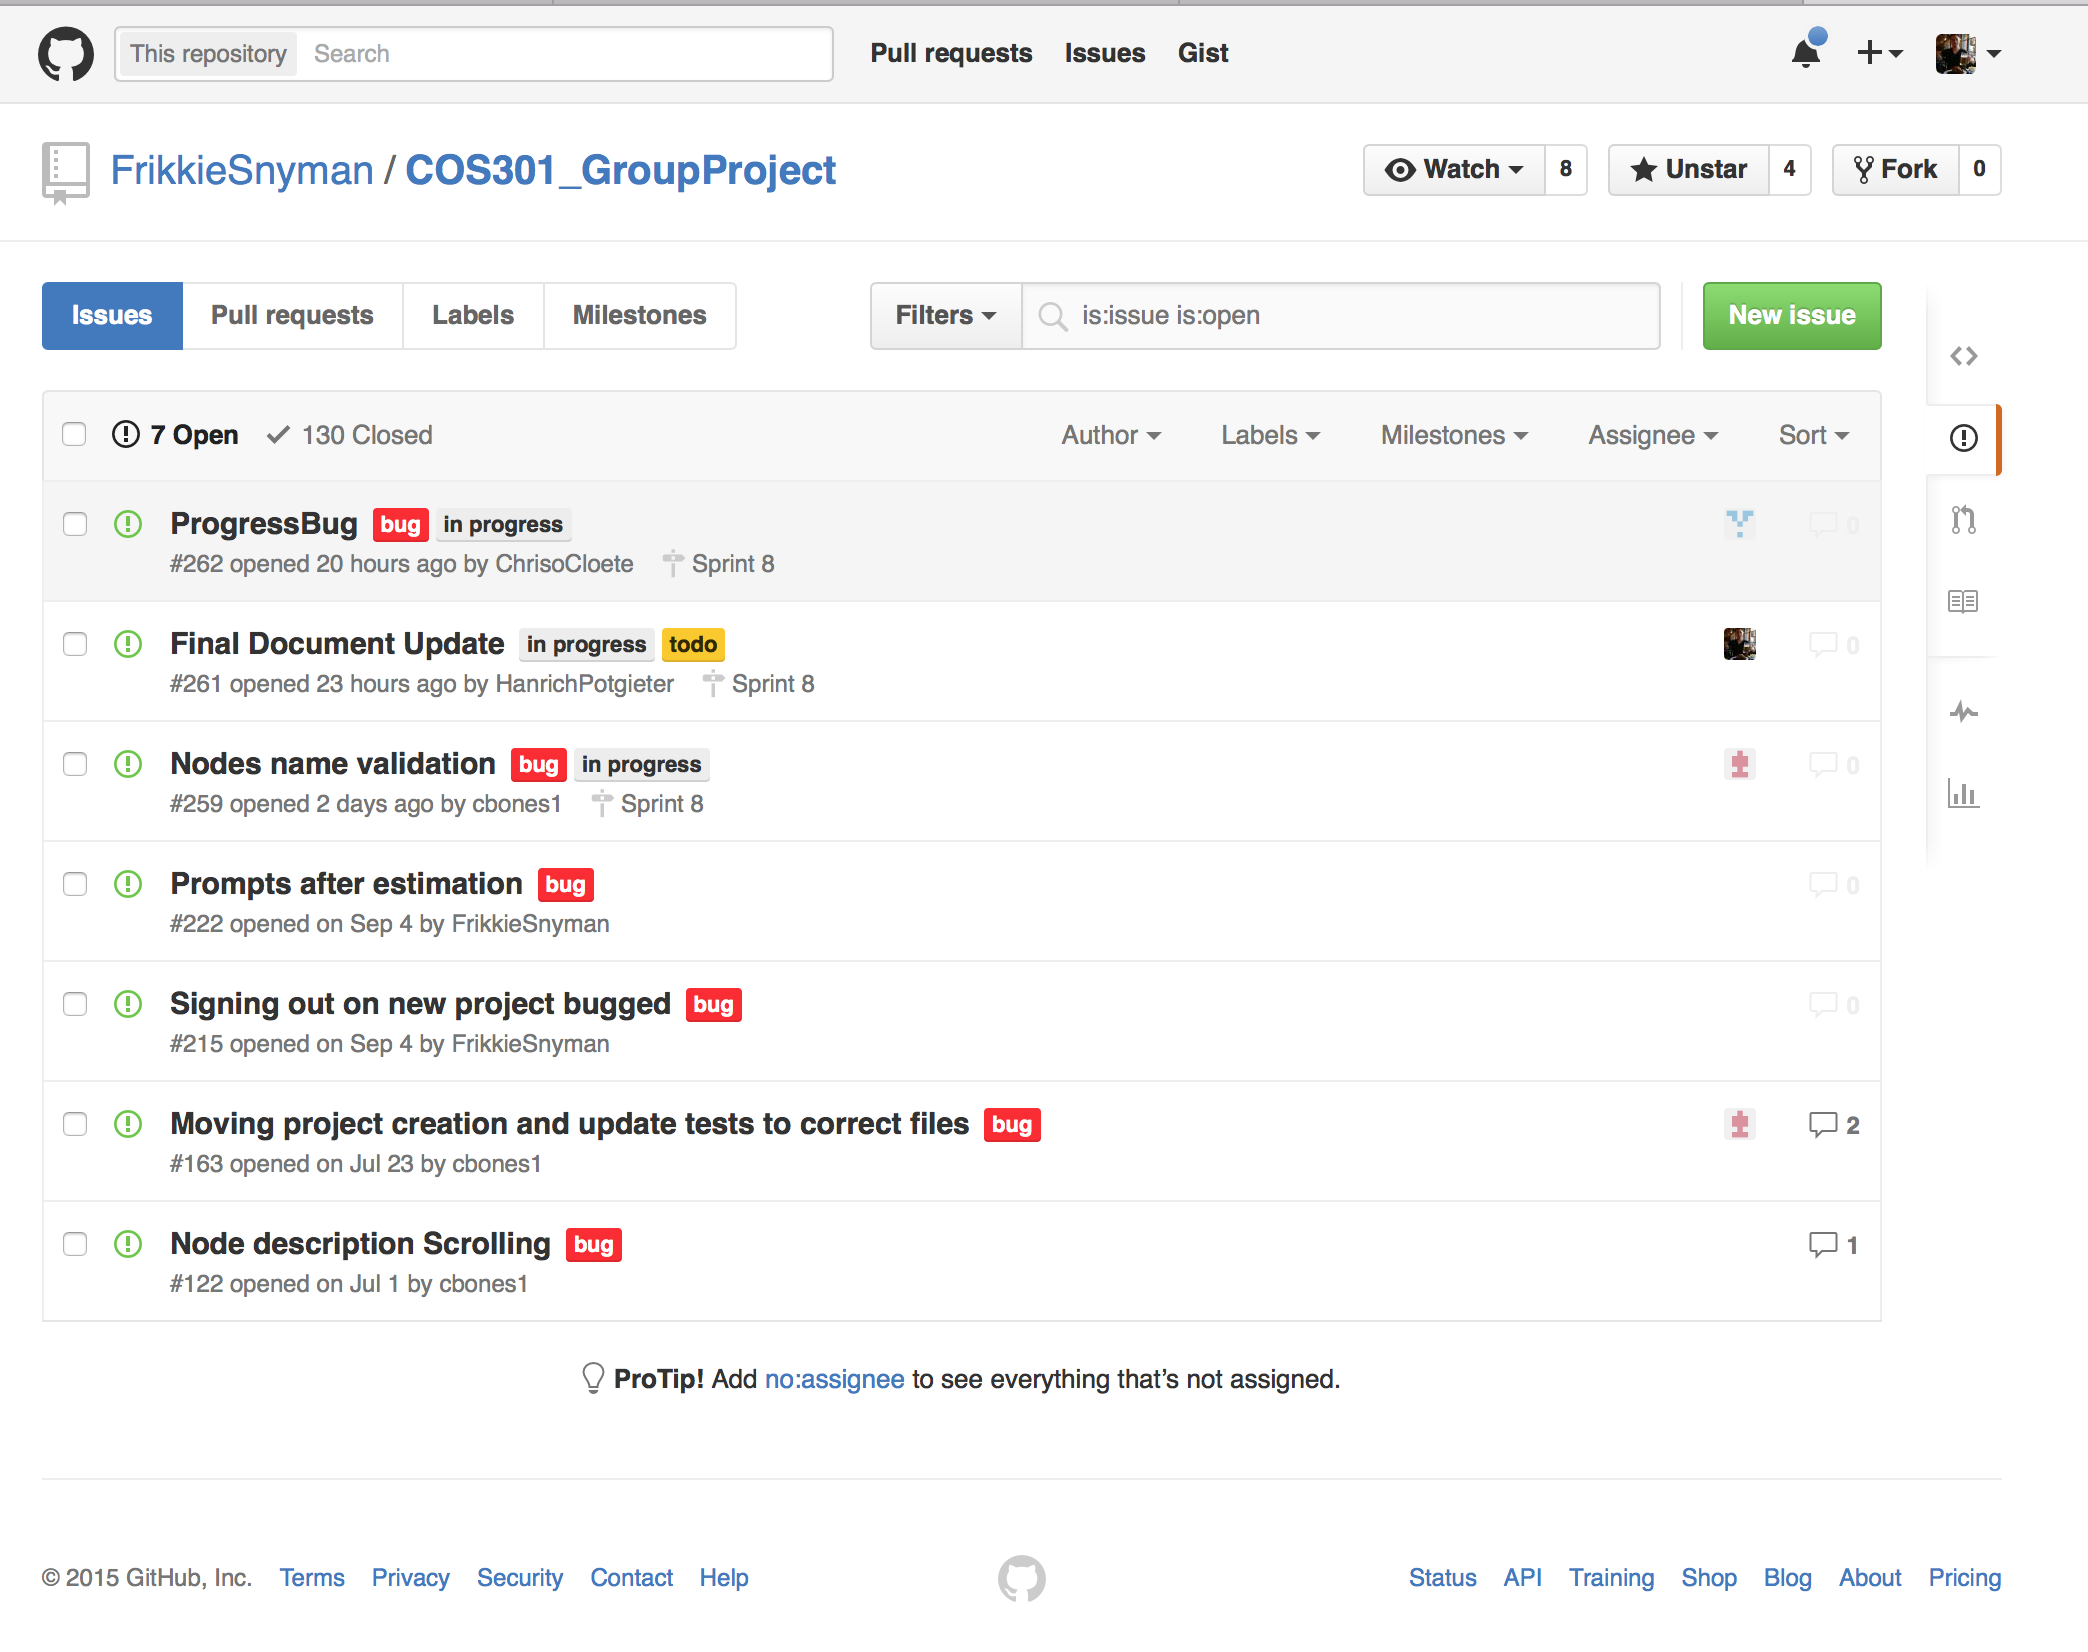
\includegraphics[width=0.5\textwidth]{gitHubIssues}}
	    	\caption{Issue Tracker}
	    	\label{fig: Issue Tracker}
   	\end{figure}
The community is always ready to support you.